%Reliability
Reliability is being explored at different layers of abstraction; from devices~\cite{Datta2014,Datta2015,Rahul2015} to memory~\cite{isca2014} to algorithms.
At a circuit-level, ~\cite{chen2015fast} uses a conditional probability approach for modeling reliability in combinational circuits.

\subsection{Introduction}
In this section, we evaluate the capabilities of a popular visual object recognition algorithm - HMAX - and exploit the potential to save 
power and reduce computational load.

\subsection{HMAX}
HMAX is a hierarchical visual object recognition model that has been used in various embedded real-time applications~\cite{Kestur2012, Maashri2012a}. 

%HMAX Expt

\subsection{Exploiting Resiliency for Power Benefits}

So far we have surveyed the landscape of vision systems that enhance the 
performance and energy efficiency of the computational fabrics. 
However, memory is an integral part of most systems today and contributes 
between 10-30\% of the overall power of embedded video systems and 
mobile phones~\cite{CarrollAaronHeiser2010}. 
The increasing memory size in new generations of embedded systems and 
the use of stacked 3D architectures that increase on-chip temperatures 
have made researchers look at saving on memory refresh energy. 
New power-efficient techniques such as Low Power Auto Self Refresh, Temperature Controlled Refresh, Refresh Pausing, Fine Granularity Refresh and Data Bus 
Inversion have been introduced in new memory standards such as 
DDR4~\cite{jedec-sdram-standards}.  

Tuning DRAM refresh based on the data characteristics has been proposed as early as 1998~\cite{islped98}.  
Many recent works have looked at tackling the increasing refresh power in other 
different ways~\cite{Liu2012, Stuecheli2010}. In ~\cite{Liu2011}, the 
authors looked at reducing refresh power on multimedia workloads. Recently, in ~\cite{iccd2014}, the authors showed that in 
real-time embedded vision applications, refresh power can dynamically be changed based on autonomously tagging data with logical labels.

%HMAX Expt
\begin{figure*}[!htb]
\centering
\begin{tabular}{@{}c@{} @{}c@{}}
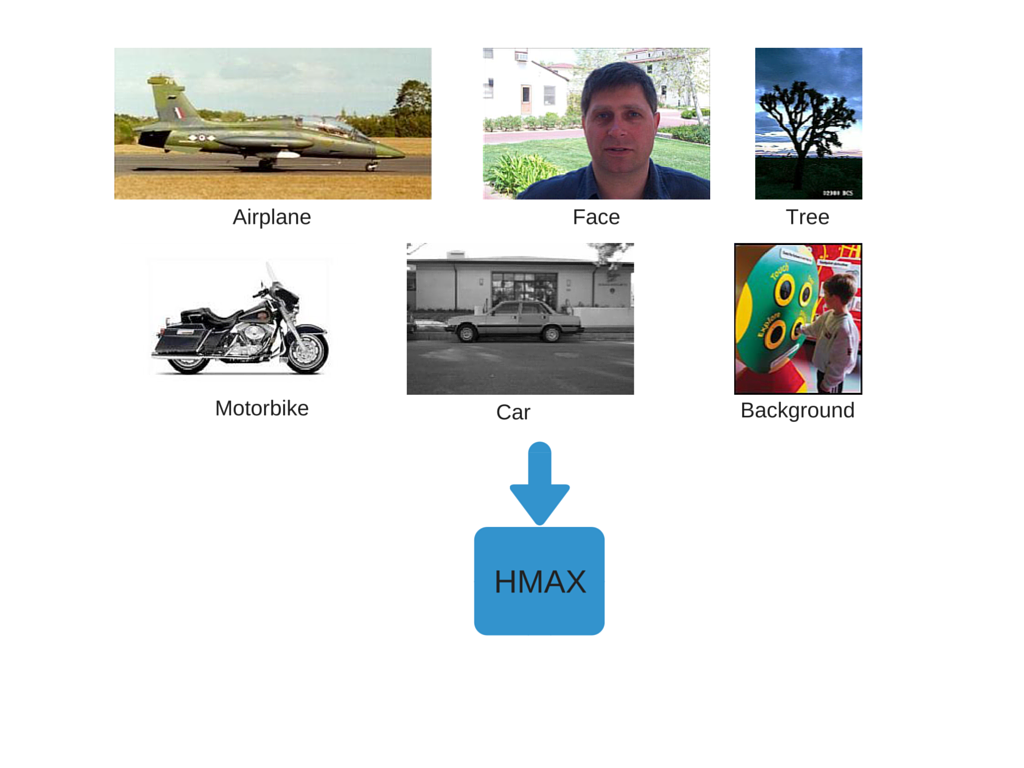
\includegraphics[width=0.45\linewidth]{./figures/hmax_reliability_a.png} & 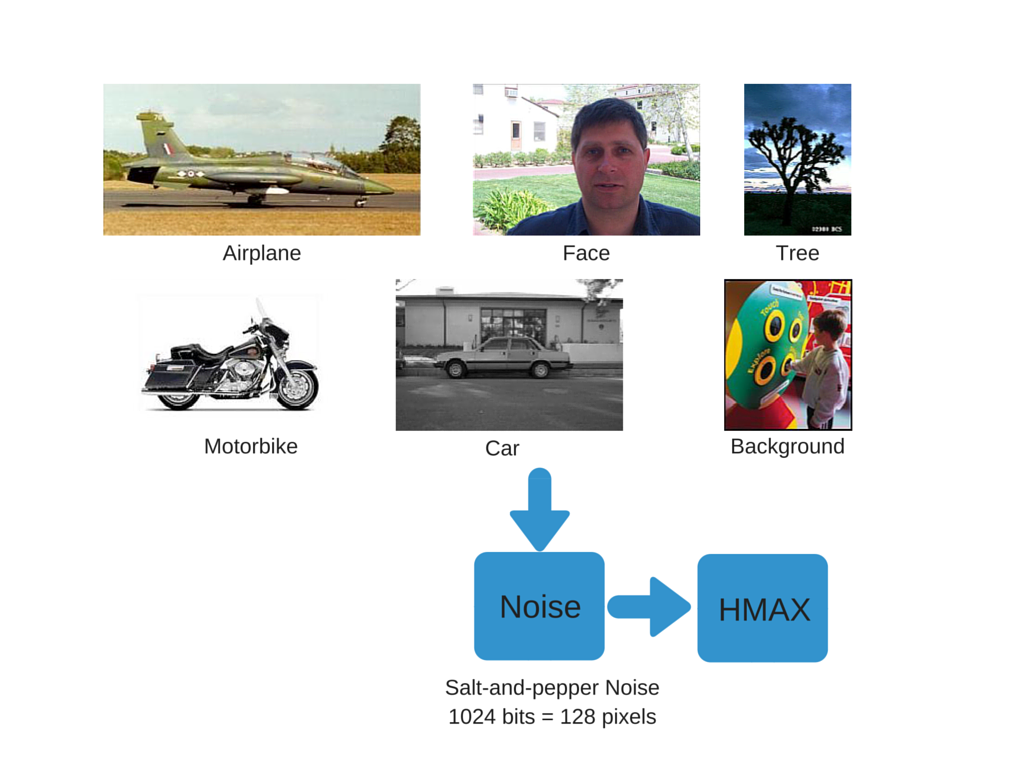
\includegraphics[width=0.45\linewidth]{./figures/hmax_reliability_b.png}\\[\abovecaptionskip]
\small (a) Baseline & \small (b) Noise
\end{tabular}
\vspace{1pt}
\caption{HMAX resilience to errors. Six classes from CalTech101 were used.}
\label{tab:hmax_reliability}
\end{figure*}

In this section, we explore the resiliency of HMAX to bit errors that can then be used to choose the refresh rate for DRAMs when these images are stored.  
Fig.~\ref{fig:hmax_pixel_sensitivity} illustrates the classification accuracy of HMAX as a function of the pixel errors introduced in each image.

%HMAX Resilience
\begin{figure}[htb!]
\vspace{0pt}
\centering
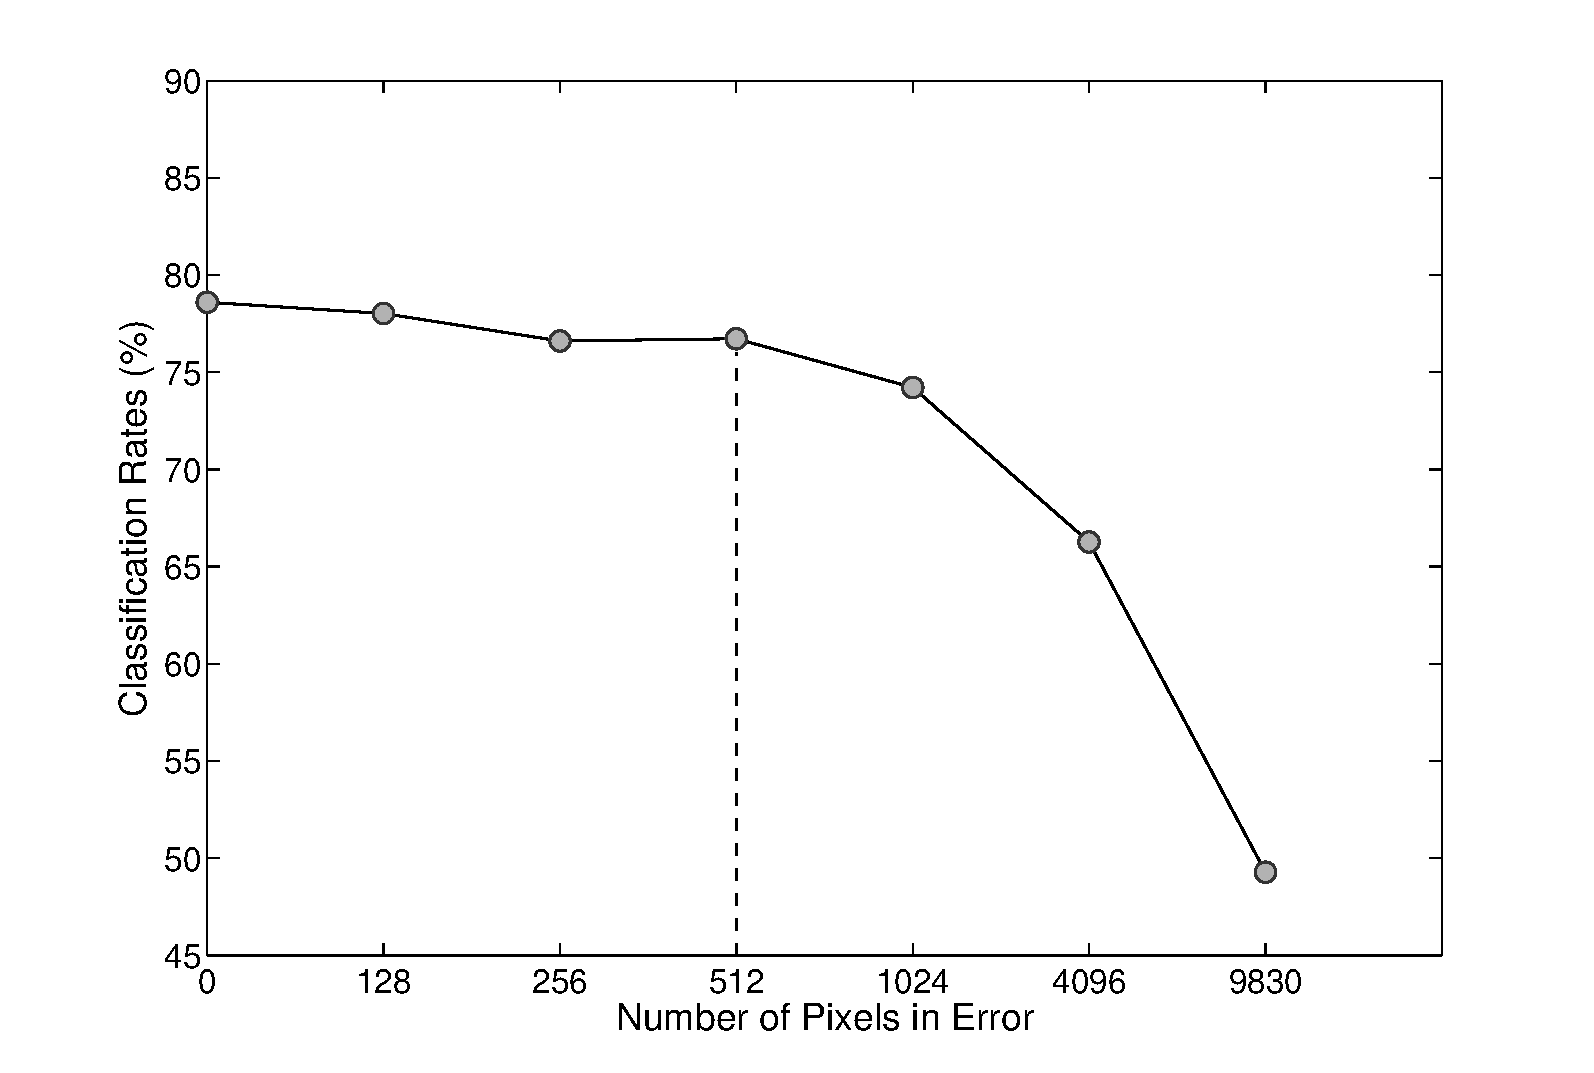
\includegraphics[width=0.99\linewidth,trim={20 20 30 20}, clip]{./figures/PixelSensitivityAnalysis.pdf}
\vspace{0pt}
\caption{HMAX resilience to errors. Six classes from CalTech101 were used.}\label{fig:hmax_pixel_sensitivity}
\vspace{0pt}
\end{figure}

\subsection{Exploiting Reseliency for Compute Benefits}
Image reconstruction is an important processing technique in image processing and computer vision applications. Most object recognition algorithms use a multi-scale 
pyramid to make it scale invariant. For example, HMAX uses an image pyramid having 11 scales (including base scale) with a scale factor of $2^{1/4}$ and 
uses a bicubic interpolation technique 
to generate the image pyramid. The input image is passed through this image pyramid before computing the ``S1'' layer of HMAX. 

%Interpolation
\begin{figure*}[!htb]
\centering
\begin{tabular}{@{}c@{} @{}c@{}}
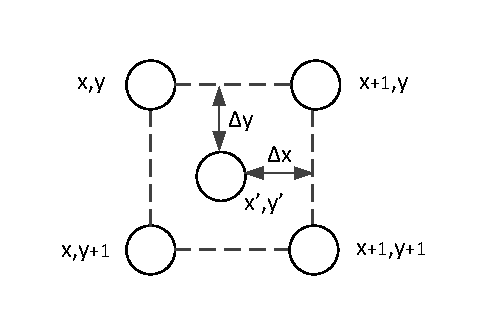
\includegraphics[width=0.3\textwidth]{./figures/bilinear.pdf} & 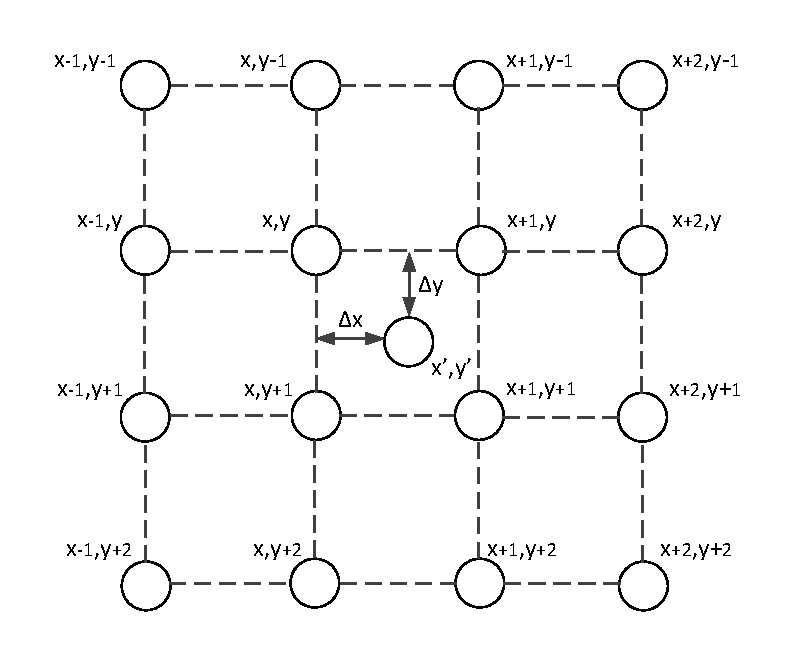
\includegraphics[width=0.5\textwidth]{./figures/bicubic.pdf}\\[\abovecaptionskip]
\small (a) Bilinear Interpolation & \small (b) Bicubic Interpolation
\end{tabular}
\vspace{1pt}
\caption{Interpolation techniques. In (a), four while in (b), 16 neighboring pixels are used for interpolation.}
\label{tab:interpolation}
\end{figure*}

Many architectures have been proposed to support linear 
and non-linear interpolation techniques~\cite{kesturdac}.

Given a pixel $I(x,y)$, an interpolated pixel $I'(x',y')$ using bilinear interpolation is given by ~(\ref{eq:1}). By definition, 
this involves computing two linear interpolation in $x$ and $y$ directions and requires eight multiplications. 
Figure~\ref{tab:interpolation}(a) illustrates an interpolated pixel using four neighboring pixels.

\begin{equation}
\begin{split}
I'(x',y') = &I(x,y) \times (1-\Delta x) \times (1-\Delta y) +\\ 
            &I(x+1,y) \times\Delta x \times (1-\Delta y) +\\ 
            &I(x,y+1) \times (1-\Delta x) \times\Delta y +\\ 
            &I(x+1,y+1) \times\Delta x \times\Delta y 
\end{split}
\label{eq:1}
\end{equation}

Using bicubic interpolation, the same interpolated pixel $I'(x',y')$ is given by ~(\ref{eq:2}) where 
$R_c$ denotes a bicubic interpolation function. The computation requires 56 multiplications in all and Figure~\ref{tab:interpolation}(b) shows the interpolated pixel 
using sixteen neighboring pixels.

\begin{equation}
\begin{split}
I'(x',y')=\sum_{m=-1}^{2}\sum_{n=-1}^{2}I(x+m,y+n)R_c(m-\Delta x)R_c(-(n-\Delta y))
\end{split}
\label{eq:2}
\end{equation}

In this section we explore the potential savings in computational work needed to be done while not compromising on accuracy. 
In the embedded version, compute resources are very costly. Saving a few resources can result in being able to 
fit a design in a particular form-factor or may cause the design to overflow into the next larger generation of devices. We explored the 
capablity of HMAX to correctly recognize objects using bilinear interpolation in the image pyramid. We used all 101 classes of CalTech101 
for this purpose. It should be noted that using the original bicubic interpolation technique, we achieve 54\% accuracy on the said dataset. This is in confirmation with the results shown in ~\cite{Mutch2008}. 
We then ran the experiment using bilinear interpolation and found the impact of this is a 1\% loss in accuracy. Also, instead of 
56 multipliers (bicubic interpolation), we would need just eight multipliers (bilinear interpolation). Table~\ref{table:compute} shows the 
results and the savings have a significant impact on area and performance of the accelerated system. 

\begin{table}[h]
\renewcommand{\arraystretch}{1.3}
\caption {Impact of Interpolation Techniques}
\label{table:compute}
\centering
\begin{tabular}{lllll}
 System & Algorithm & Accuracy & Multipliers\\\hline
 HMAX	& Bicubic   & 54\% & 56\\\hline
 HMAX   & Bilinear  & 53\% & 8\\\hline
\end{tabular}
\end{table}
